\documentclass{article}
\usepackage{amssymb}
\usepackage{amsmath}
\usepackage{centernot}
\usepackage{algpseudocode}
\usepackage{graphicx}
\usepackage[margin=1in]{geometry}
\setlength{\parindent}{0in}

\begin{document}

\title{EE360C: Lab 1}
\author{Joshua Dong (jid295)}
\date{\today}
\maketitle

\subsection*{a) Existence Proof}
We will show that a weakly stable matching exists using the Gale-Shapely
algorithm where landlords will reject applicant tenants of equal preference if
their apartment is already paired. It may be shown that our algorithm is
equivalent to Gale-Shapely but with equal preferences being silently ordered
according to the order of the apartment or tenant listings.
\\\\
To prove the existence of a stable matching, we first show that the algorithm
terminates and produces a matching $S$. Then we will show that $S$ is weakly
stable.
\\\\
All apartments are either paired or free. Suppose a tenant applies to all
apartments but is rejected every time. Then all apartments must be paired.
Since the number of tenants and apartments are equal and no tenant has
two apartments, this would imply all tenants have found an apartment,
a contradiction. Thus our algorithm always produces a valid matching.
\\\\
Let there be $n$ apartments and tenants. Then the number of pairings is
$n^2$, the number of edges of a complete bipartite graph with edges
representing matchings. Each round of our algorithm eliminates one edge.
$n^2$ is finite. Thus our algorithm terminates.
\\\\
Let the resulting match of our algorithm be $S$. If an arbitrary tenant prefers
another apartment to their current apartment, then they must have been
rejected by that apartment previously. If they were rejected, then their
preferred apartment must be paired with a tenant the landlord preferred
equally or more. Then that apartment does not prefer the tenant over its
current tenant. Since the selected tenant was arbitrary, this applies to all
tenants. Then we conclude that no unstable matchings exist and $S$ is weakly
stable.
\\\\
Since our program produces a weakly stable matching and always terminates,
there must exist a weakly stable matching for any $n$ apartments and tenants.


\newpage
\subsection*{b) Algorithm}
We provide the algorithm used in the previous section:

\begin{algorithmic}
\While {$\exists \> T$ where $T$ is free}
    \State {$A \gets$ top choice apartment for $T$}
    \State {$A$ is removed from the list of choices for $T$}
    \If {$A$ is free}
        \State {$(T, A)$ are paired}
    \Else
        \State {$T' \gets$ match for $A$}
        \If {$A$ prefers $T$ to $T'$}
            \State {$T'$ is unpaired from $A$}
            \State {$(T, A)$ are paired}
        \EndIf
    \EndIf
\EndWhile
\end{algorithmic}


\subsection*{c) Correctness}
We already established that our algorithm terminates. Since our algorithm is
equivalent to the tenant-optimal Gale-Shapely algorithm, we know that the
resultant matching of our algorithm is weakly stable as proven in the
Existence Proof section. 
\\\\
Our program terminates and always produces correct output. Therefore, it is 
totally correct.


\subsection*{d) Runtime Complexity}
We already showed that the problem is bounded by $n^2$ possible matchings. Our
algorithm always removes a possible matching in the last statement in the
while loop. Then there are a maximum of $n^2$ iterations of our loop.
\\\\
Inside the while loop, there are no other loops since all of our checks and
statements are $O(1)$: checking if a given apartment is free is $O(1)$,
getting the match of a given apartment is $O(1)$, preference checking is
$O(1)$, and pairing or unpairing is $O(1).$\footnote{In our implementation,
we use HashMaps, which are $O(n)$ if there are collisions for every lookup.
However, this is so rare that $\Theta(1)$ is a more accurate representation
of HashMap lookups and insertions.} We accomplish $O(1)$ execution per
iteration with the creation of maps and bimaps before we enter the loop.
\\\\
Since our loop iterates at most $n^2$ times and each iteration of the loop
costs at most $O(1)$ lookups, deletes, or assignments, we conclude that our
algorithm is $O(n^2).$\footnote{Due to our use of HashMap as explained above,
$O(n^3)$ is the actual complexity of our algorithm. $O(n^2)$ is a
more accurate upper bound, practically. In any case, our algorithm is of
polynomial time complexity.}


\subsection*{e) Brute Force}
In a brute force solution, we would produce all matchings and filter for
stable matchings.
\\\\
Let $n$ be the number of apartments or tenants. There are
$n!$ possible unique matchings between apartments and tenants. There are $n^2$
possible pairings between apartments and tenants since this is the number of
edges in a complete bipartite graph of parameters $n$ and $n$. For each
different matching need to check all possible pairings to validate stability,
thus a brute force algorithm would be require at most $n! \cdot n^2$ checks.
We may simplify and say the brute force solution is $O(n^n)$.


\newpage

\subsection*{f) Graphs}
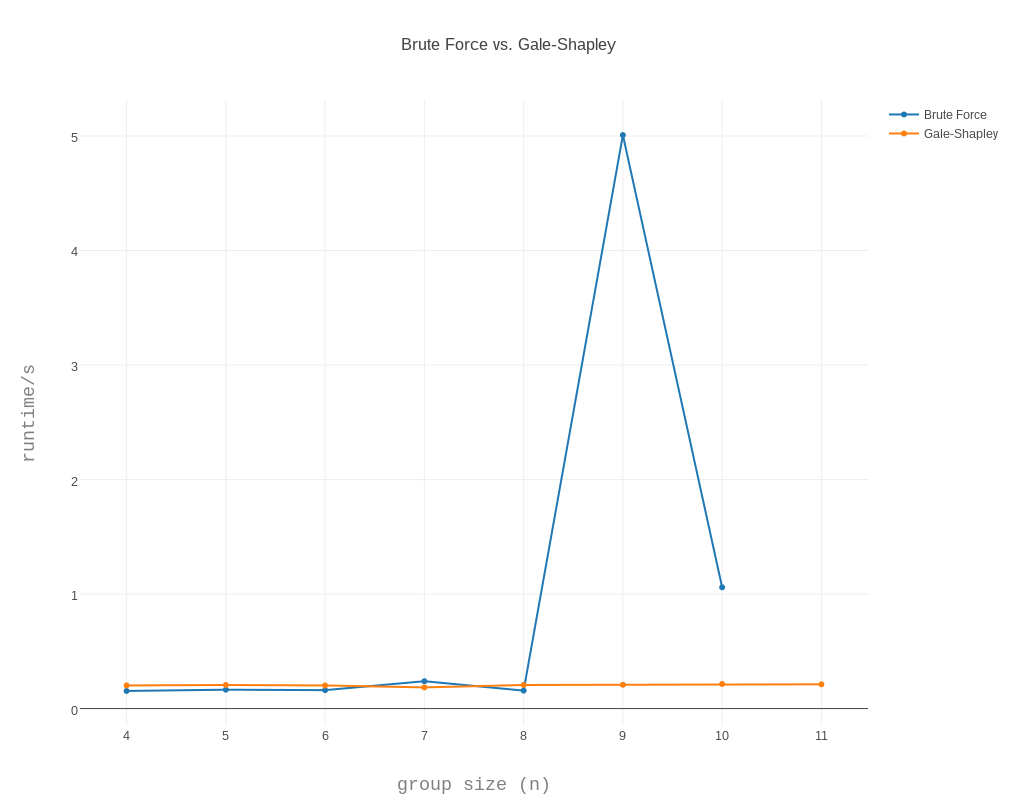
\includegraphics[width=\linewidth]{../graph/plot.png}

Runtime of the brute force algorithm was unstable and increased to very large
values after the size of the input exceeded 10. The Gale-Shapely algorithm was
mostly consistent and did not increase much, with at most a weak linear
increase.


\end{document}
